Como o exercício é uma ordenação, podemos apenas utilizar um método simples de
vetores, logo cada vetor vai ser um dia da semana e cada dia da semana vai ter
seus parâmetros para serem inseridas, por exemplo: as pessoas que tem o nome
que começam com a letra A,B,C e D, vão ficar no vetor de domingo, podendo ser
apenas ser implementado como um if ou case dentro de um for para fazer a
verificação de todo o vetor de nomes.

\begin{center}
    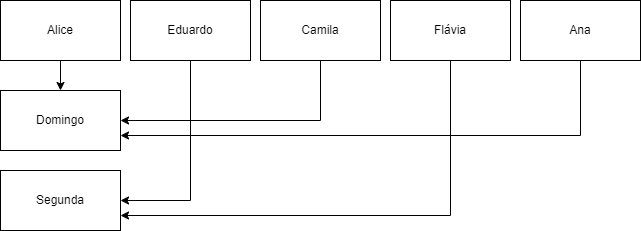
\includegraphics[scale=0.5]{lista/lista-ed.png}
\end{center}

Complexidade total: $O(n)$.
